\documentclass[10pt, graphics, aspectratio=169, table]{beamer}
\usepackage{hyperref}
\usepackage{booktabs}
\usepackage[normalem]{ulem}

% -- Change to this year's color! --
\definecolor{ese}{RGB}{89, 71, 179}
\newcommand{\ra}{$\Rightarrow$\ }

\usetheme{metropolis}
\setbeamercolor{frametitle}{bg=ese}

\title{Regex - Regular expressions}
\author{Eric Wolf}
\date{ESE \the\year{}}
\institute{Nerd::101 - ESE - ifsr - TU Dresden}
\titlegraphic{\hfill
\includegraphics[height=2cm]{../logo}}

\begin{document}
    \maketitle

    \begin{frame}{Outline}
        \tableofcontents
    \end{frame}


    \section{Introduction}
        \begin{frame}{Motivation}
        \begin{columns}
            \column{0.55\textwidth}
                \emph{Information is often represented as text}
                \begin{itemize}
                    \item automation \ra 200 MB of email, one address
                    \item representation \ra address is unknown
                    \item storage \ra email is not always accessible as files
                \end{itemize}
                \textbf{We need a standardized pattern language}
            \column{0.45\textwidth}
                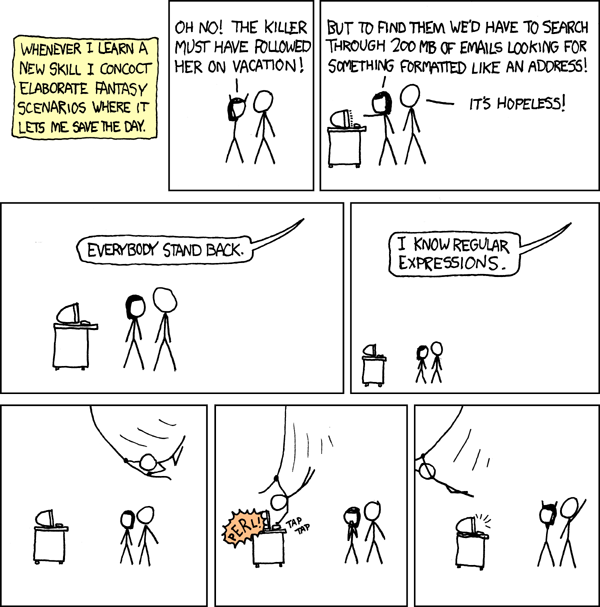
\includegraphics[width=\textwidth]{img/xkcd_usage.png}
                \center\tiny\url{https://xkcd.com/208}
        \end{columns}
    \end{frame}

    \begin{frame}{Solution}
        Enter: \textbf{Regular expressions}
        \begin{itemize}
            \item multiple use cases \ra match, search, replace, \ldots
            \item simple and compact syntax \ra can be entered in small search boxes
            \item inspired by formal language theory \ra abstract enough to allow for different implementations
            \item standardized (sort of) \ra Perl and Posix, wide application support
        \end{itemize}
    \end{frame}


    \section{Basic Syntax}
    \begin{frame}{Literals}
        \begin{itemize}
            \item all characters (except metacharacters) are matching themselves
            \item metacharacters (\{\}[]()\textasciicircum\$.|*+?\textbackslash) can be escaped using \textbackslash
            \item some escaped literals have special meaning (for example groups)
            \item some metacharacters match text too
        \end{itemize}
        \begin{center}
            \begin{tabular}{cl}
                \toprule
                Character & Pattern \\
                \midrule
                . & any single character (sometimes excluding newlines) \\
                \textasciicircum & start of the string or line (does not consume characters) \\
                \$ & end of the string or line (does not consume characters) \\
                \bottomrule
            \end{tabular}
        \end{center}
    \end{frame}

    \begin{frame}[fragile]{Literal examples}
        \begin{center}
            \begin{tabular}{cl}
                \toprule
                Regular expression & Match \\
                \midrule
                \verb|a| & a \\
                \verb|\.| & . \\
                \verb|\\| & \textbackslash \\
                \bottomrule
            \end{tabular}
        \end{center}
    \end{frame}

    \begin{frame}{Groups}
        \begin{itemize}
            \item match a single character of some set
            \item {[\ldots]} matches a single character of the ones contained
            \item {[\textasciicircum\ldots]} matches all characters except the ones contained
            \item can contain multiple ranges like a-zA-Z (letters) or 0-9 (numbers)
            \item metacharacters lose their meaning inside (escaping still works)
            \item not to be confused with (), which behaves like in math
        \end{itemize}
    \end{frame}

    \begin{frame}[fragile]{Group examples}
        \begin{center}
            \begin{tabular}{cl}
                \toprule
                Regular expression & Match \\
                \midrule
                \verb|[ab]| & a or b \\
                \verb|[^ab]| & every single character except a or b \\
                \verb|[ab^]| & a or b or \textasciicircum \\
                \verb|[a.b]| & a or b or . \\
                \verb|[a-z!.0-9?]| & any single lowercase letter, number or !?. \\
                \verb|\d| & any match of \verb|[0-9]| \\
                \verb|\s| & any whitespace \\
                \verb|\w| & any match of \verb|[a-zA-Z0-9_]| \\
                \bottomrule
            \end{tabular}
        \end{center}
    \end{frame}


    \section{Nesting}
    \begin{frame}{Concatenation}
        \begin{itemize}
            \item regular expressions can be concatenated
            \item the concatenation matches text which is a concatenation of two matches
        \end{itemize}
        \emph{Please use multiline features of your implementation before creating giant one-liners!}
    \end{frame}

    \begin{frame}[fragile]{Concatenation examples}
        \begin{center}
            \begin{tabular}{cl}
                \toprule
                Regular expression & Match \\
                \midrule
                \verb|ab| & ab \\
                \verb|a.b| & a<any single character>b \\
                \verb|[1-9]\d| & any two digits not starting with zero \\
                \bottomrule
            \end{tabular}
        \end{center}
    \end{frame}

    \begin{frame}{Alternation}
        \begin{itemize}
            \item \ldots|\ldots{} is the Alternation of two regular expressions
            \item it matches text which is a match of one of the sub-expressions
            \item be careful when concatenating: alternation has a higher precedence than concatenation!
        \end{itemize}
    \end{frame}

    \begin{frame}[fragile]{Alternation examples}
        \begin{center}
            \begin{tabular}{cl}
                \toprule
                Regular expression & Match \\
                \midrule
                \verb!a|bc!  & a or bc \\
                \verb!(a|b)c! & ac or bc \\
                \verb!a|bc|e! & a or bc or e \\
                \bottomrule
            \end{tabular}
        \end{center}
    \end{frame}

    \begin{frame}{Quantifiers}
        \begin{itemize}
            \item match a preceding regular expression multiple times
            \item exact amount is implementation dependant (most implementations match as much as they can)
        \end{itemize}
        \begin{center}
            \begin{tabular}{cl}
                \toprule
                Quantifier & Amount \\
                \midrule
                ? & zero or one \\
                * & zero or more \\
                + & one or more \\
                \{n\} & n \\
                \{min,\} & at least min \\
                \{,max\} & at most max \\
                \{min,max\} & at least min and at most max \\
                \bottomrule
            \end{tabular}
        \end{center}
    \end{frame}

    \begin{frame}[fragile]{Quantifier examples}
        \begin{center}
            \begin{tabular}{cl}
                \toprule
                Regular expression & Match \\
                \midrule
                \verb!^(0|-?[1-9]\d*)$!  & integers \\
                \verb!^Home\ssweet(\sHome\ssweet)*\sHome$! & Home sweet \ldots{} Home \\
                \verb!^\s*(#|$)! & beginning of non-code lines (Python) \\
                \bottomrule
            \end{tabular}
        \end{center}
    \end{frame}


    \section{Application}
    \begin{frame}{grep}
        \begin{itemize}
            \item grep is a command-line utility for searching files for lines with regular expressions
            \item it is preinstalled on most Linux systems
            \item the initial release was in 1973
        \end{itemize}
        \begin{center}
            \begin{tabular}{ll}
                \toprule
                Command & Use \\
                \midrule
                grep PATTERN FILE & search for lines of FILE containing matches of PATTERN \\
                grep -v PATTERN FILE & search for lines not containing matches of PATTERN \\
                grep -E PATTERN FILE & enable the metacharacters \{\}()|+? \\
                grep -c PATTERN FILE & count lines instead of printing them \\
                grep -o PATTERN FILE & only print matched part of matching lines \\
                grep -R PATTERN DIRECTORY & search all files in a directory recursively \\
                \bottomrule
            \end{tabular}
        \end{center}
    \end{frame}

    \begin{frame}[fragile]{Python}
        \begin{itemize}
            \item support is available in the \href{https://docs.python.org/3/library/re.html}{re} module
            \item implements multiple advanced extensions (not python specific)
            \item multiple modes of matching
            \item allows access to parts of a match matched by a specific (math) group with \href{https://docs.python.org/3/library/re.html#re.Match.group}{Match.group}
        \end{itemize}
        \begin{center}
            \begin{tabular}{cl}
                \toprule
                Function & Mode \\
                \midrule
                \href{https://docs.python.org/3/library/re.html#re.search}{search} & search for the first match anywhere in the string \\
                \href{https://docs.python.org/3/library/re.html#re.match}{match} & match the beginning of the string \\
                \href{https://docs.python.org/3/library/re.html#re.fullmatch}{fullmatch} & match the entire string \\
                \bottomrule
            \end{tabular}
        \end{center}
    \end{frame}

    \begin{frame}{Pitfalls}
        \begin{columns}
            \column{0.55\textwidth}
                \begin{itemize}
                    \item regular expressions are designed to be compact \ra dont scale well to larger expressions
                    \item have been augmented for greater power \ra no replacement for a full parser
                    \item are often implemented by backtracking \ra quadratic worst case performance
                \end{itemize}
                \emph{With great power comes great responsibility}
            \column{0.45\textwidth}
                
\includegraphics[width=\textwidth]{img/xkcd_problem.png}
                \center\tiny\url{https://xkcd.com/1171}
        \end{columns}
    \end{frame}


    \section{What to do next}
    \begin{frame}{What to do next}
        \begin{itemize}
            \item try to write your own expressions!
            \item debug complex ones on sites like \href{https://regex101.com}{regex101.com}!
            \item \sout{fear} solve \href{https://regexcrossword.com/}{regex crosswords}!
        \end{itemize}
        \begin{center}
            
\includegraphics[scale=0.3]{img/unlimited_power.png} \\
            \tiny\href{https://star-wars-memes.fandom.com/wiki/Unlimited_power!}{have fun!}
        \end{center}
    \end{frame}
\end{document}